% !TeX root = ../main.tex
% Add the above to each chapter to make compiling the PDF easier in some editors.

\chapter{Results}\label{chapter:results}
In this chapter, the following experiments are performed.
For all experiments the test data is used.
Then, an inverse problem is generated.
This is run x times.

\section{Latent Dimension}
The latent dimension of the VAE has an effect of the representational error.
With an increase of the latent dimension, the VAE is able to represent more information.
This means the range of the generator is bigger.
The representational error, i.e. the error observed if the complete field is sensed, is smaller.
However, with a bigger range, the search for a point becomes more difficult.
This results in the following [to fill].
\begin{figure}[h!]
    \centering
    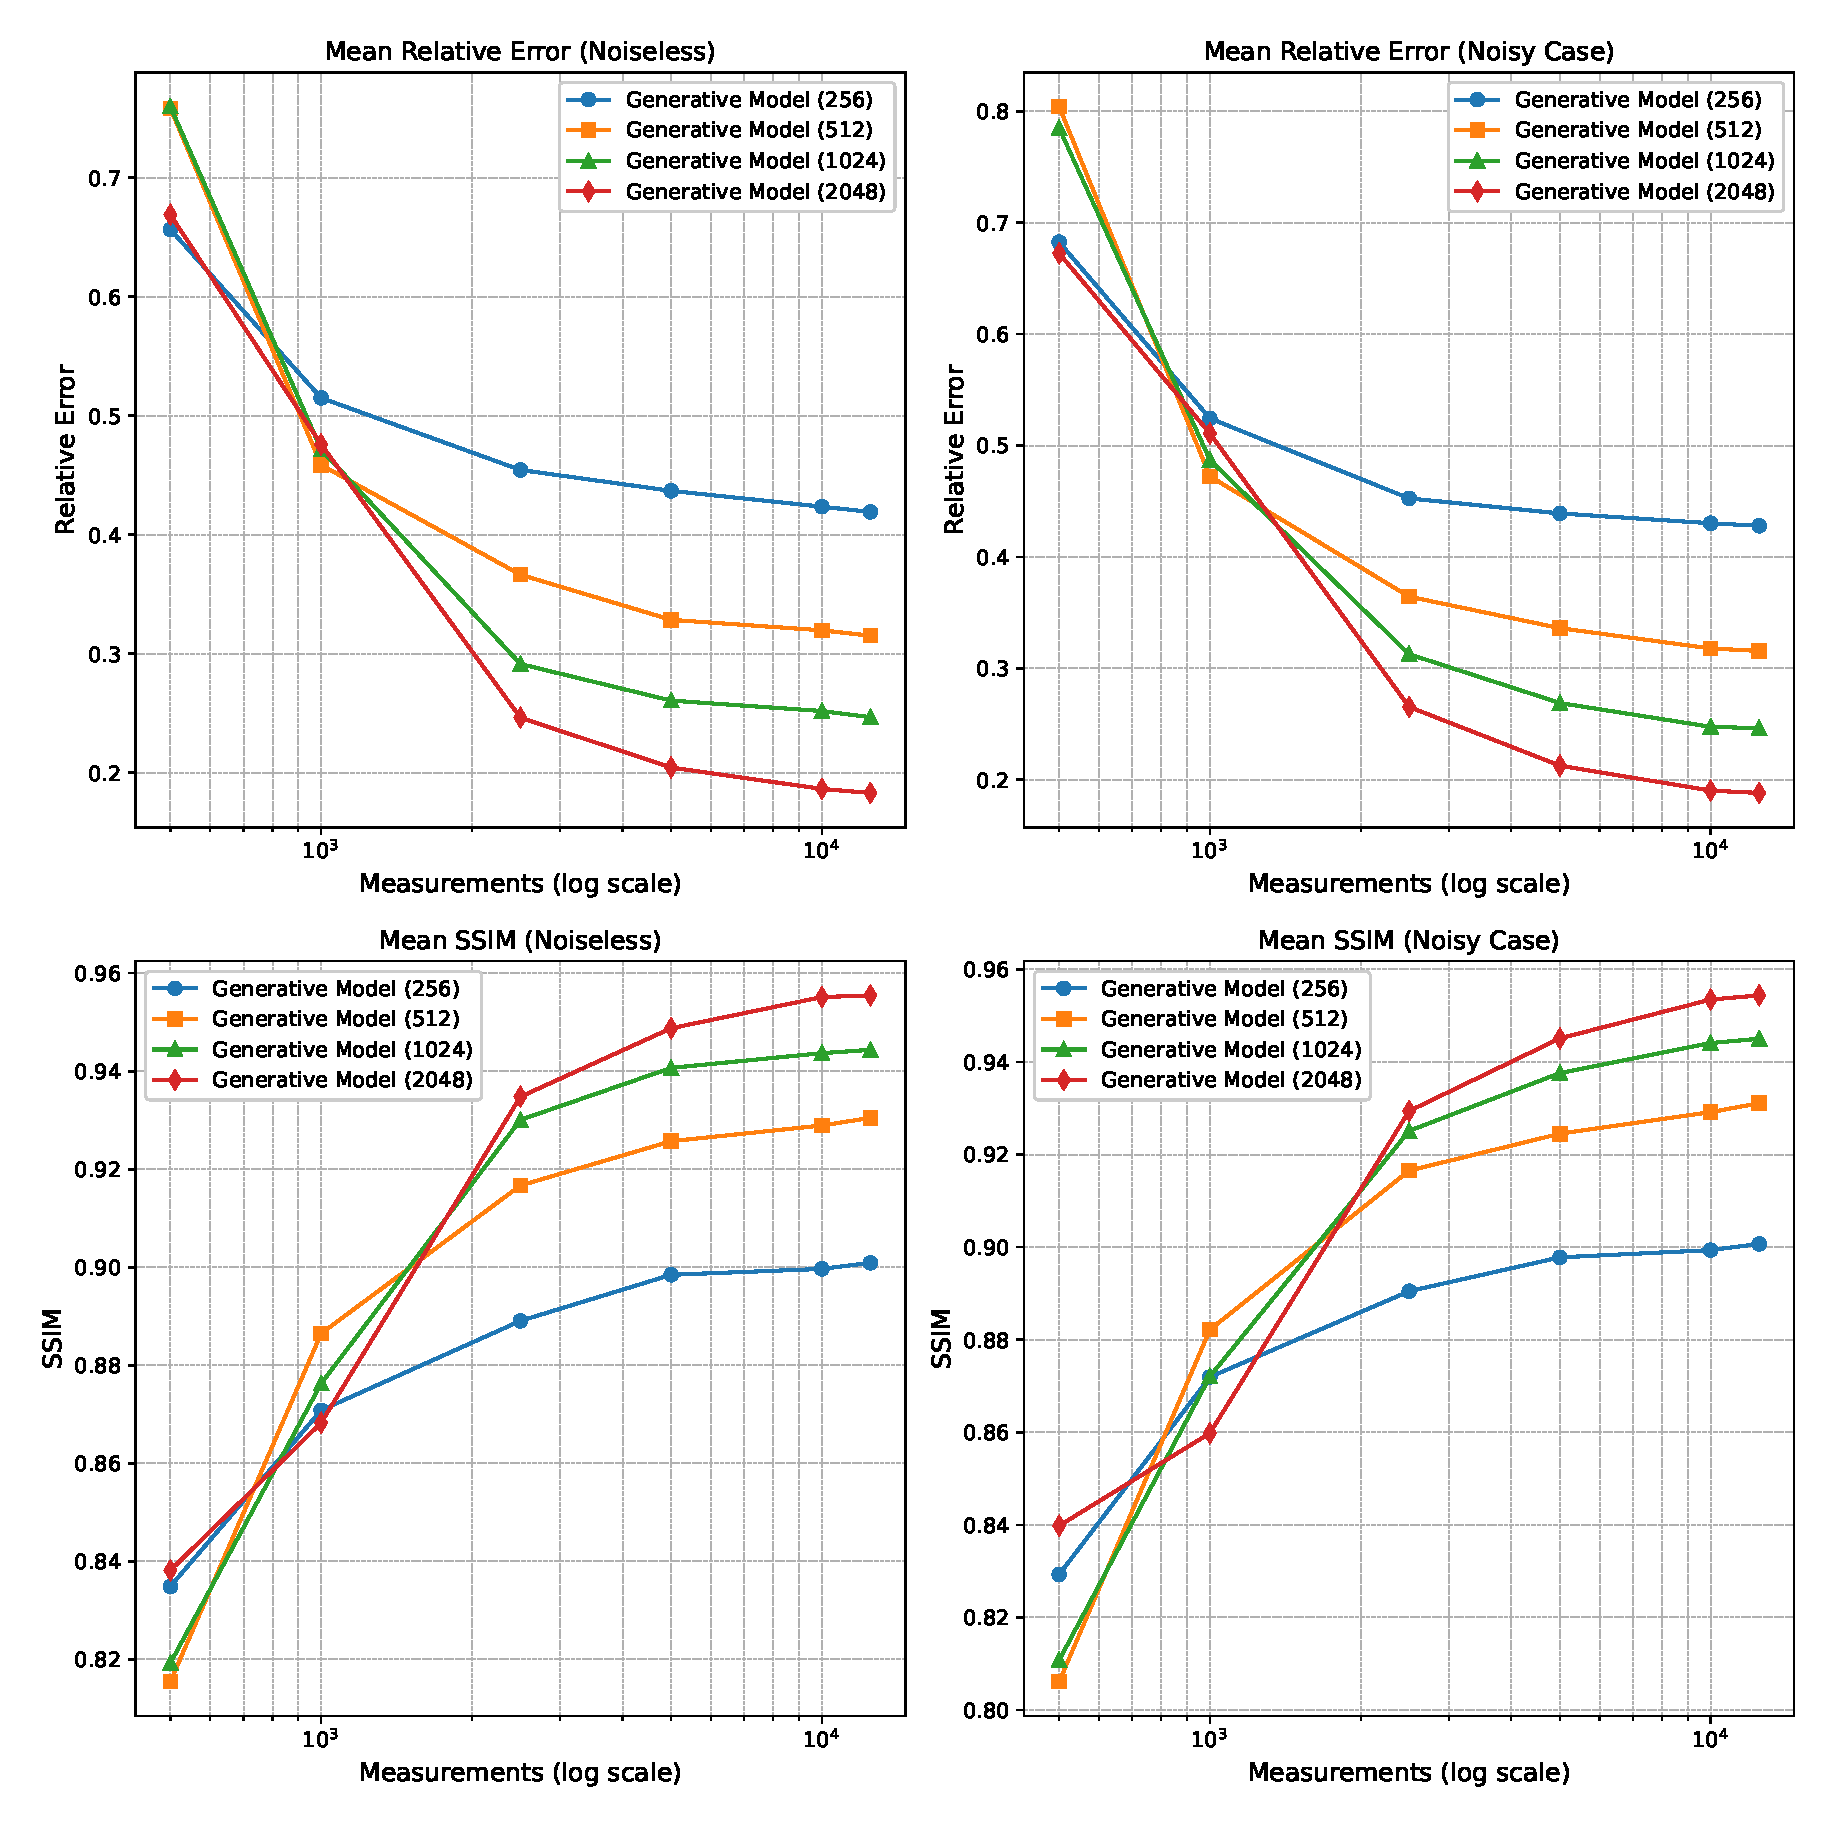
\includegraphics[width=\textwidth]{figures/06_results/latent_dimension.eps}
    \caption{Latent Dimensions}
\end{figure}
A smaller latent dimension will have a smaller error for few measurements
A bigger latent dimension will have a smaller error for many measurements.

\section{Fine-tuned Models vs Base Models}
\begin{figure}[h!]
    \centering
    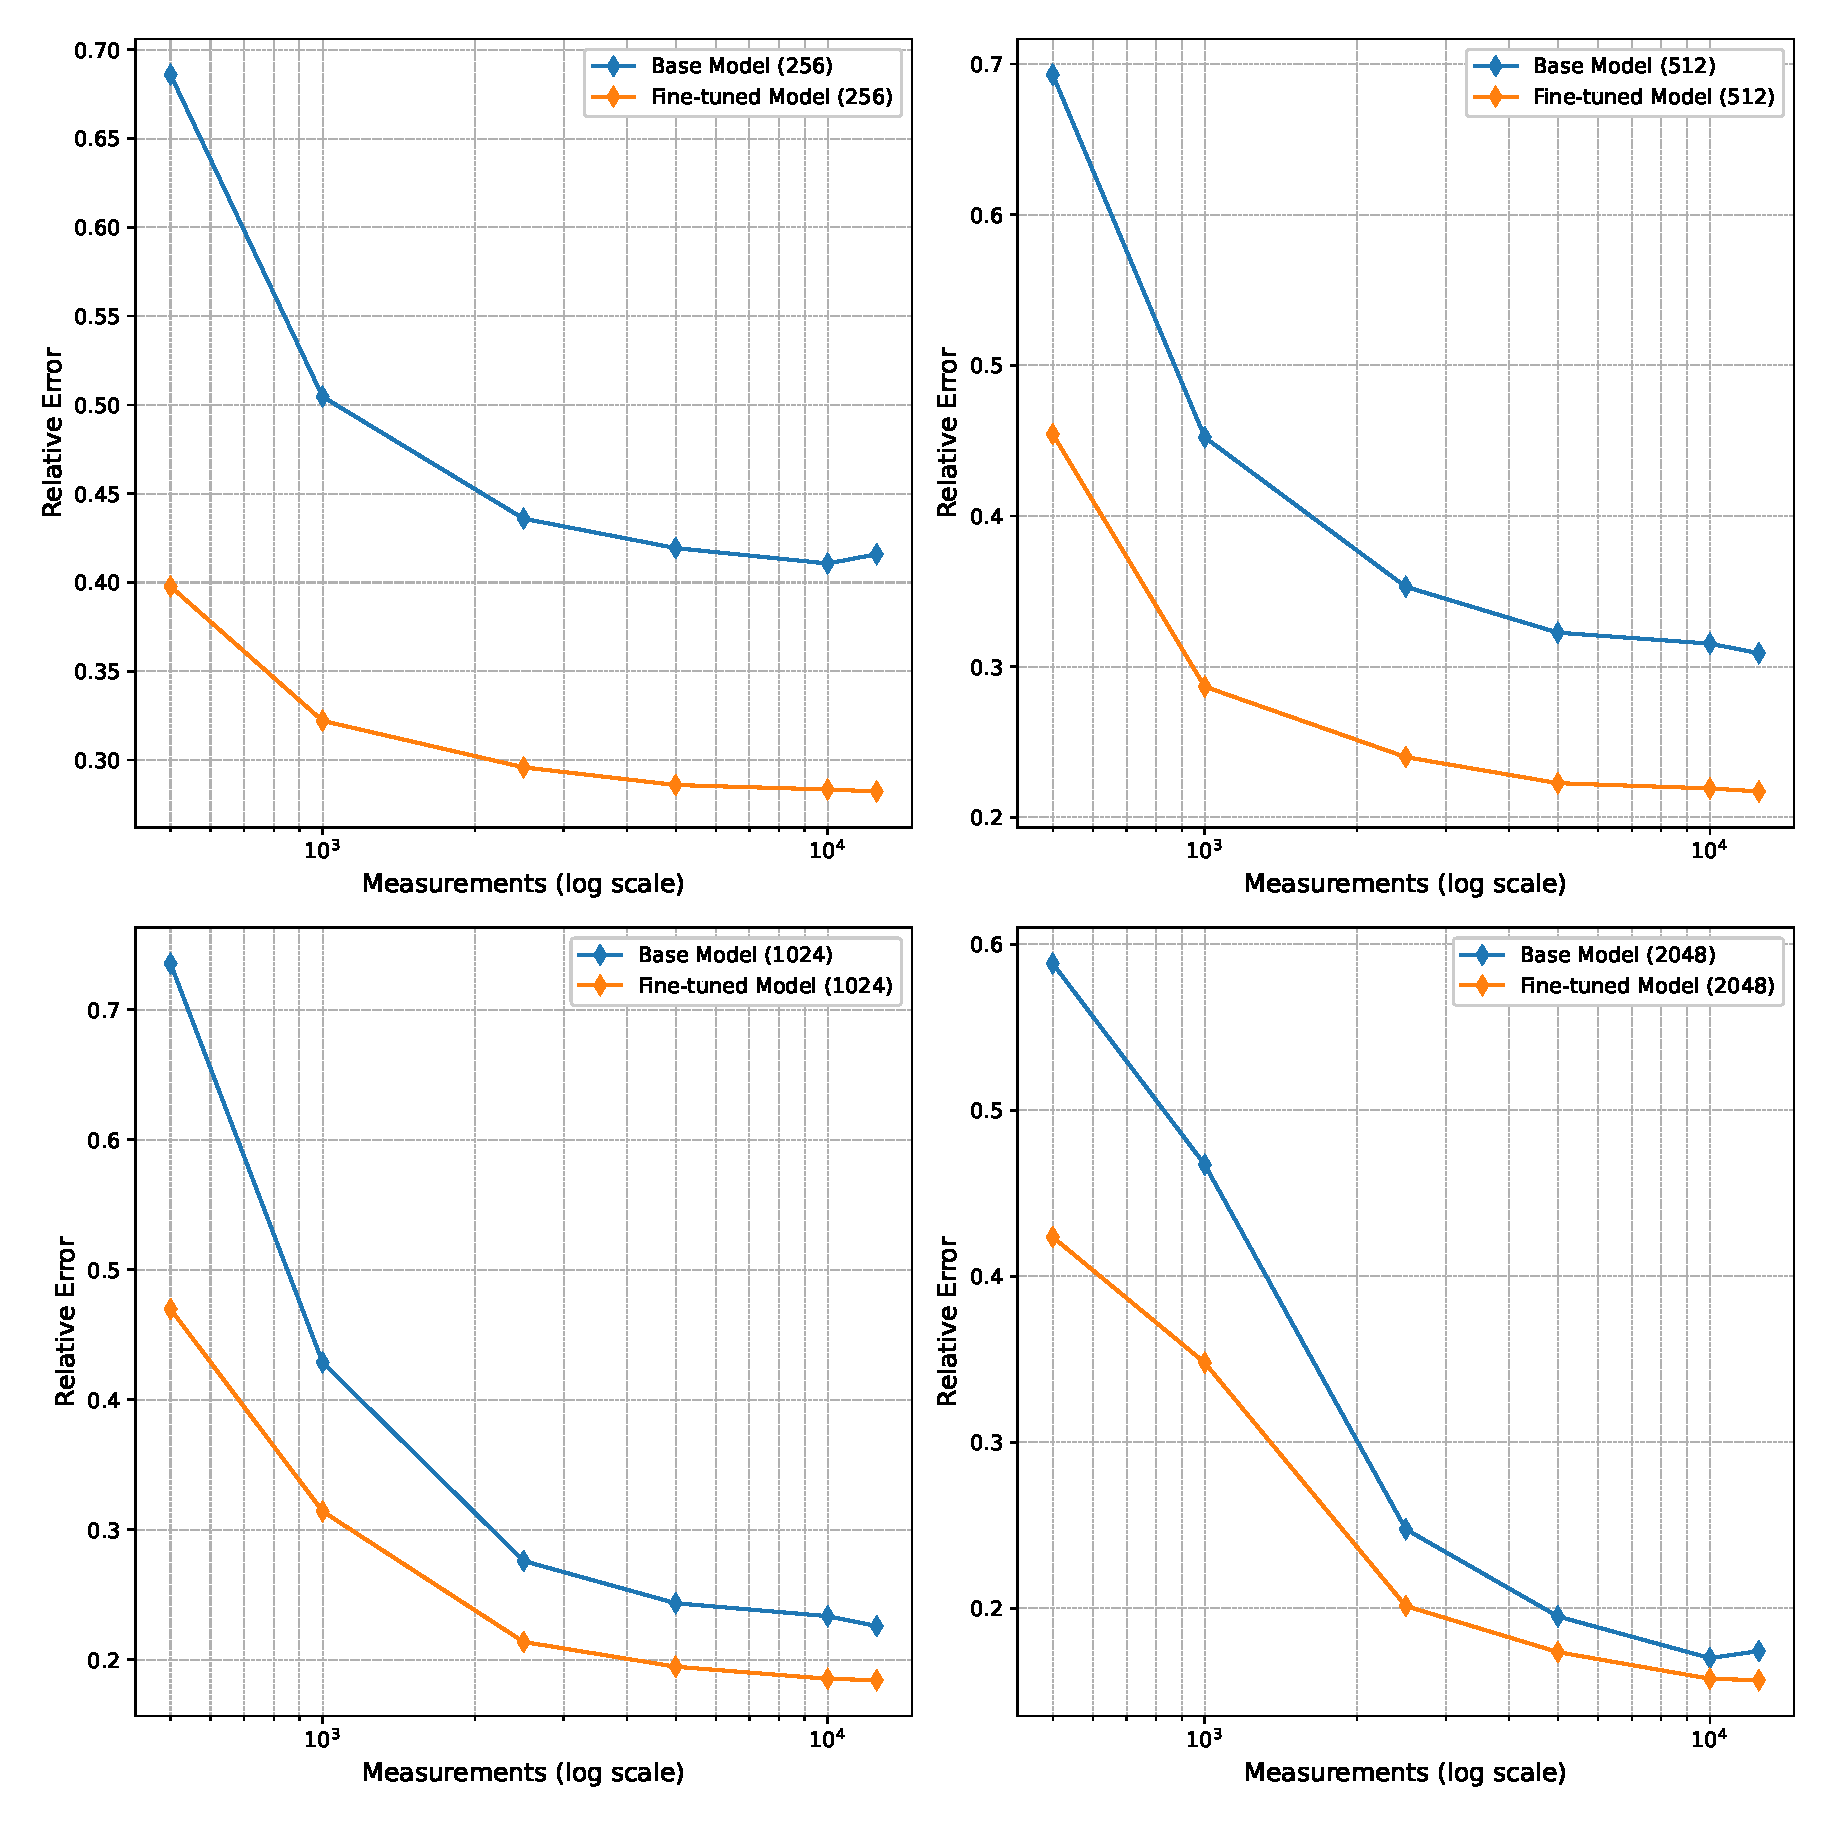
\includegraphics[width=\textwidth]{figures/06_results/fine_tuned_zuerich.eps}
    \caption{Results for Fine-tuned Model Zurich}
\end{figure}
The other plots can be seen in the appendix.
Overall, they follow the same trend.

\section{Generative Models vs Lasso}
\begin{figure}[h!]
    \centering
    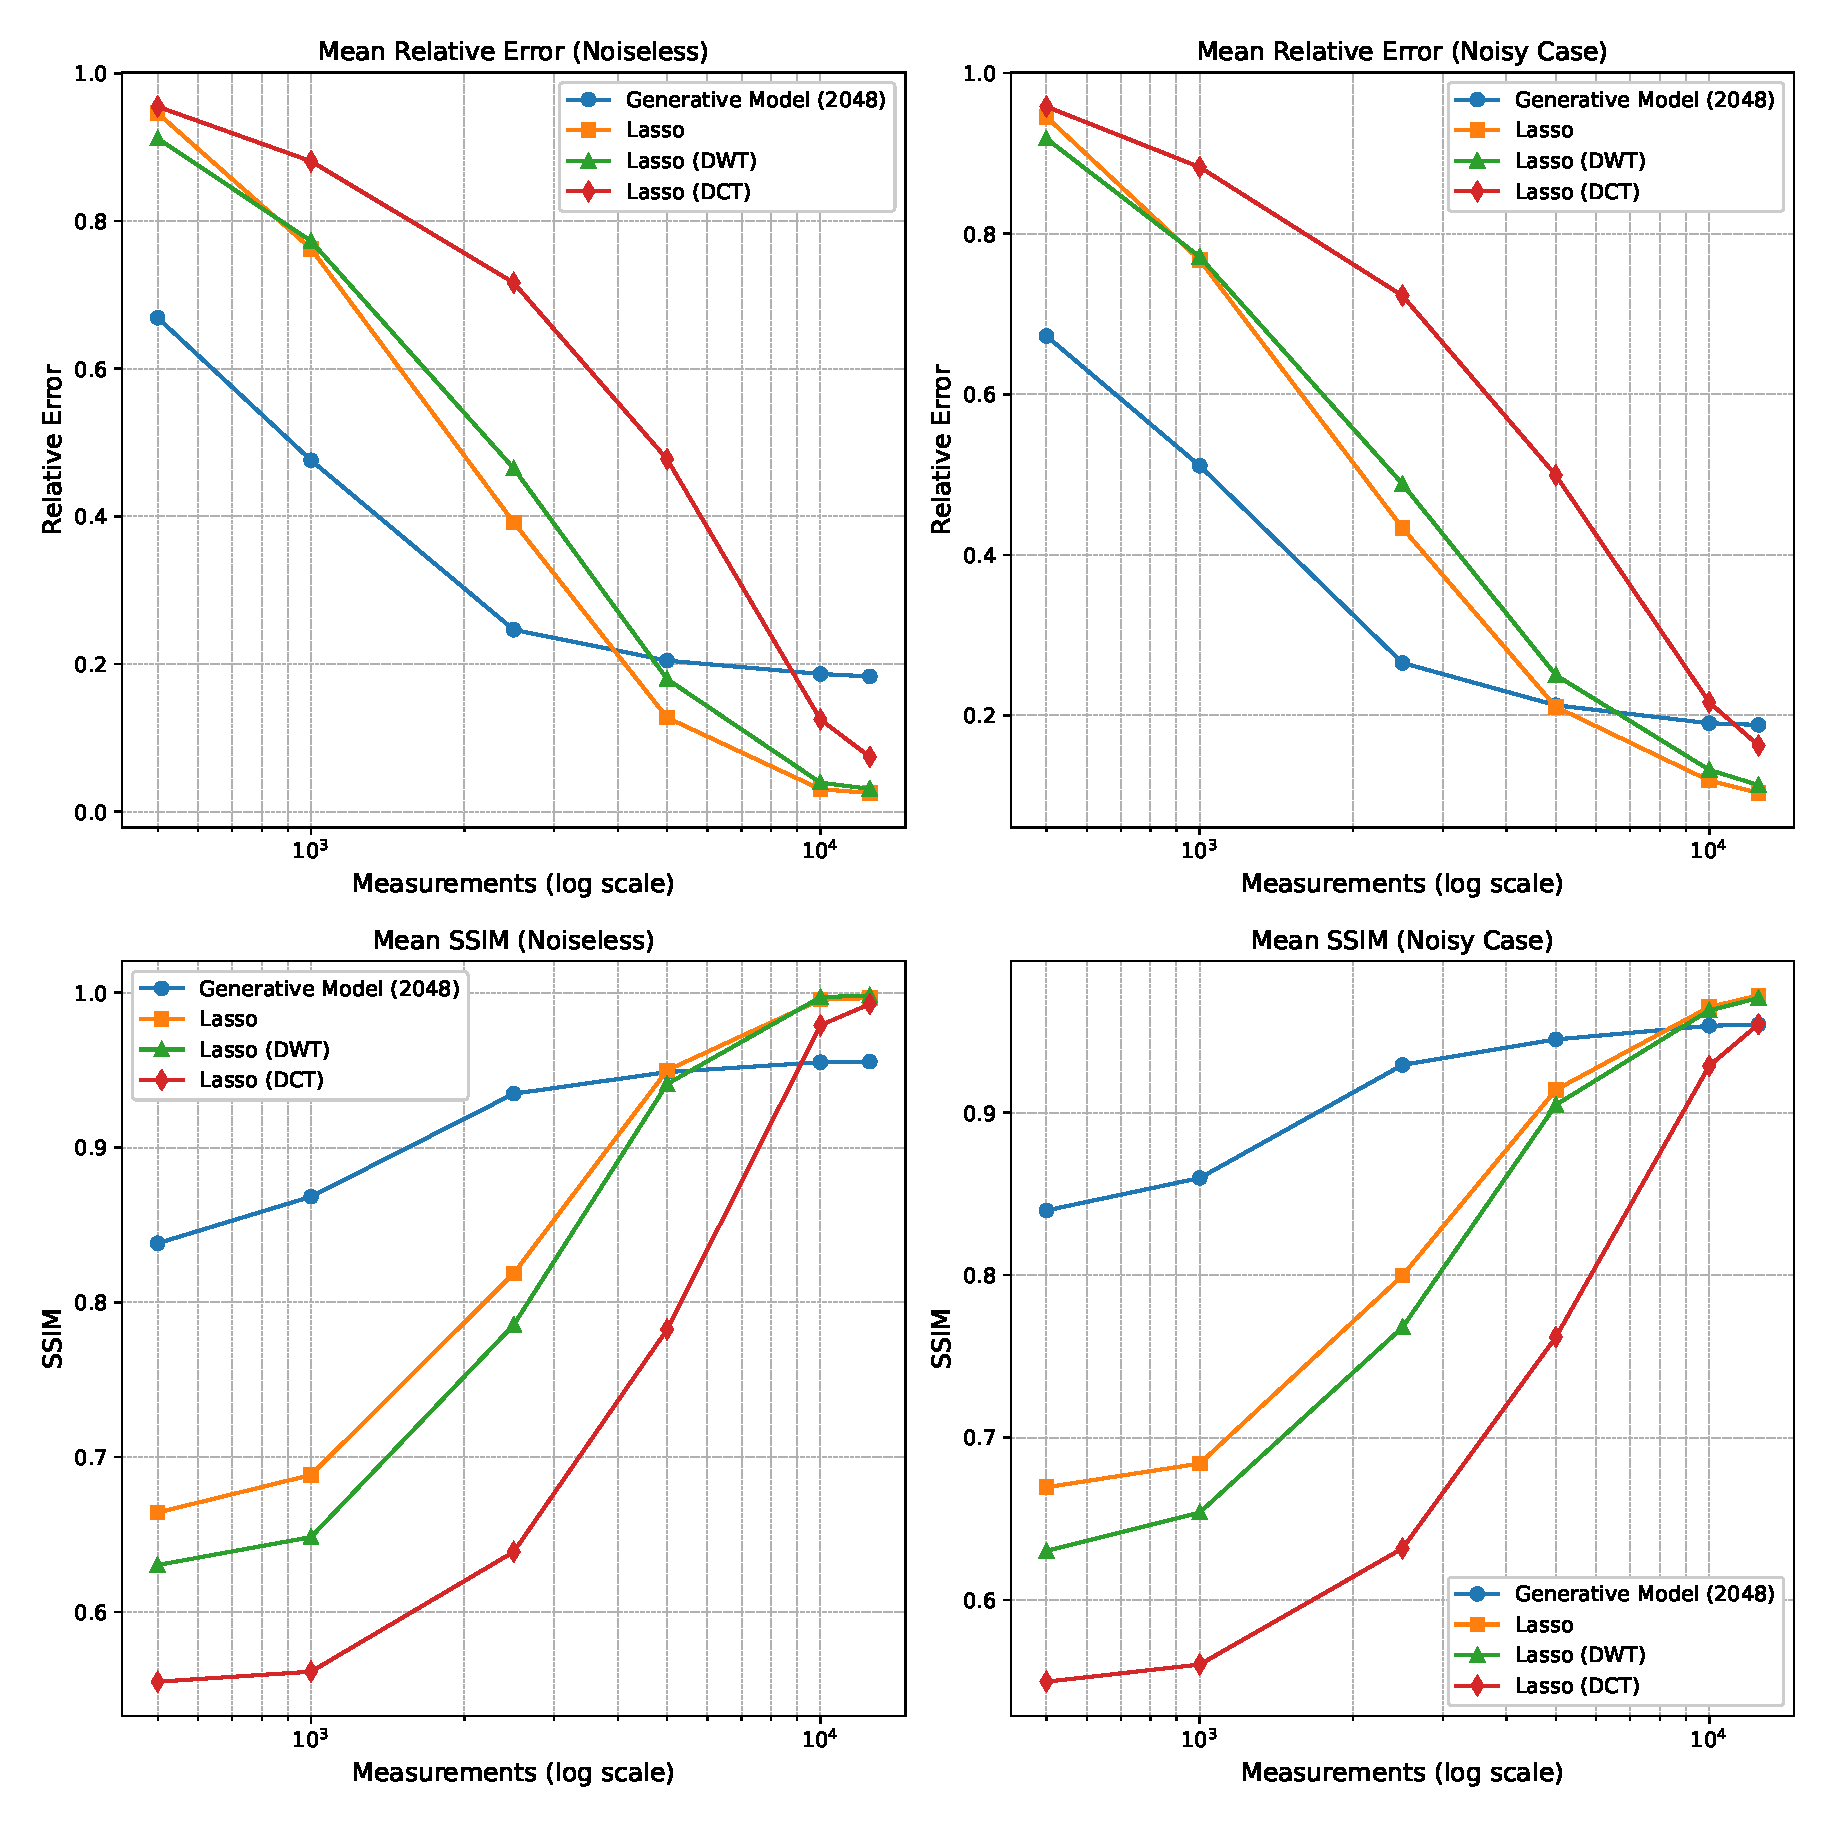
\includegraphics[width=\textwidth]{figures/06_results/gen_vs_lasso.eps}
    \caption{Generative Model vs Lasso}
\end{figure}
Make a graph that keeps num measurements fixed and only varies the noise.

\section{Atmospheric Inversion}
The first run is an SNR plot.
For this run, the artifical footprints from Benjis paper are taken.
Jzst like in his paper, $3\%$ of unknowns measuement stations are used, i.e. 30.
Each measuement station takes $50$ measurements.
The signal to noise ratio is altered.
For each SNR, 3 problems are created to get better sampling.

Make a plot that has x axis snr and y axis relative error just like in Benjis plot.
Do this for the 3 cities.

The second run is an example to qualitatively assess the performance.
The situation is very favorable with a low to moderate SNR of 20dB.
The chosen city is Munich.
The example run was done with 13 measurement stations.
Each measurement station takes 50 measurements.
This results in 750 measurements.
The guassian plume simulation was run for a predefined wind field.
This wind field covers ~180 degrees.
\begin{figure}
    \centering
    \begin{subfigure}[b]{0.32\textwidth}
        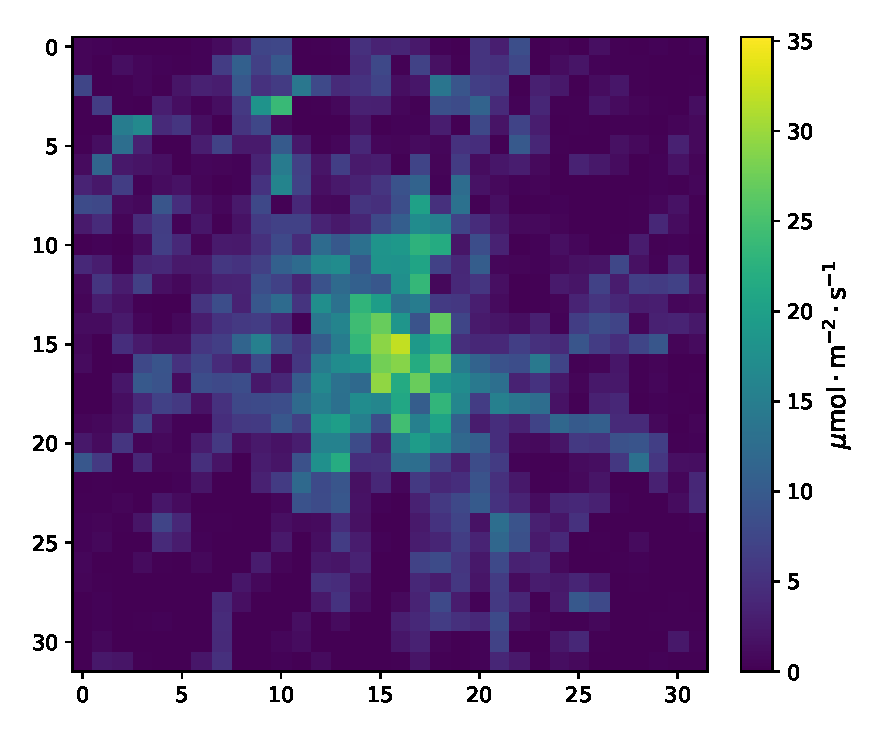
\includegraphics[width=\textwidth]{figures/06_results/gaussian_plume_example/munich/target.eps}
        \caption{Target Munich}
    \end{subfigure}
    \begin{subfigure}[b]{0.32\textwidth}
        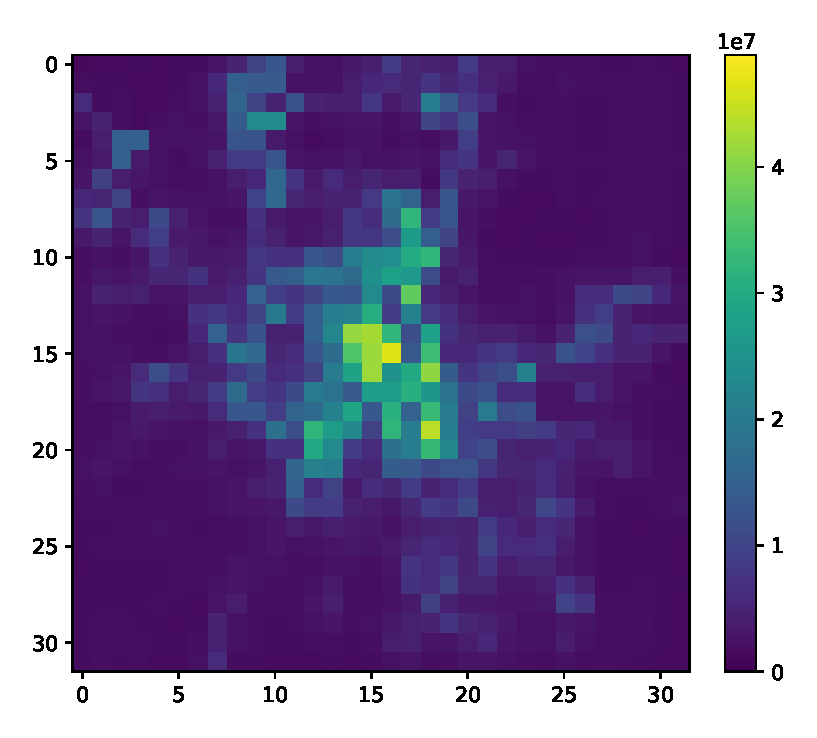
\includegraphics[width=\textwidth]{figures/06_results/gaussian_plume_example/munich/gen_2048_fine_tuned_20_db.eps}
        \caption{Gen 2048 Fine-tuned}
    \end{subfigure}
    \begin{subfigure}[b]{0.32\textwidth}
        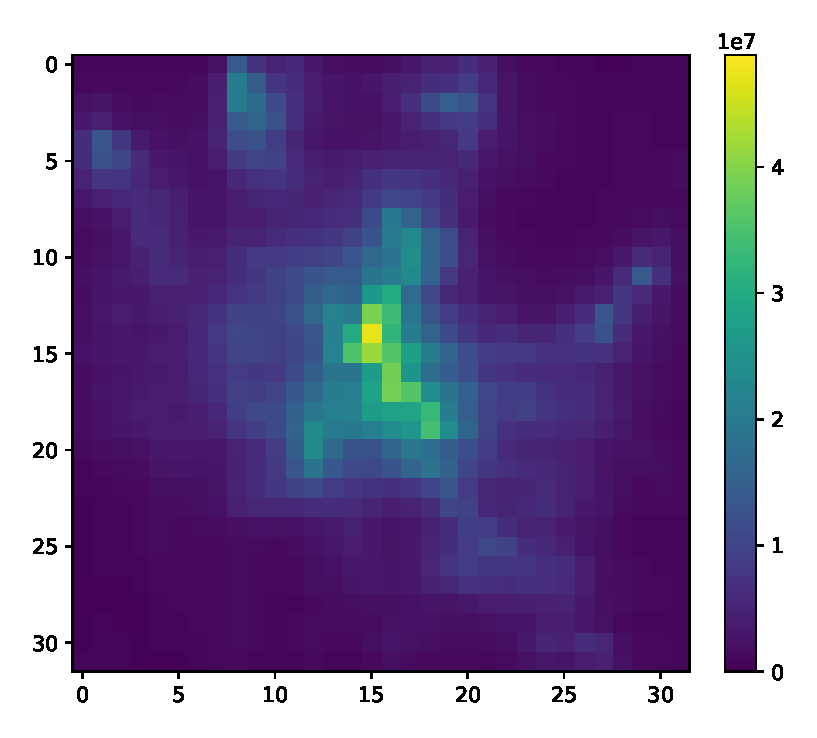
\includegraphics[width=\textwidth]{figures/06_results/gaussian_plume_example/munich/gen_2048_20_db.eps}
        \caption{Gen 2048}
    \end{subfigure}
    \begin{subfigure}[b]{0.32\textwidth}
        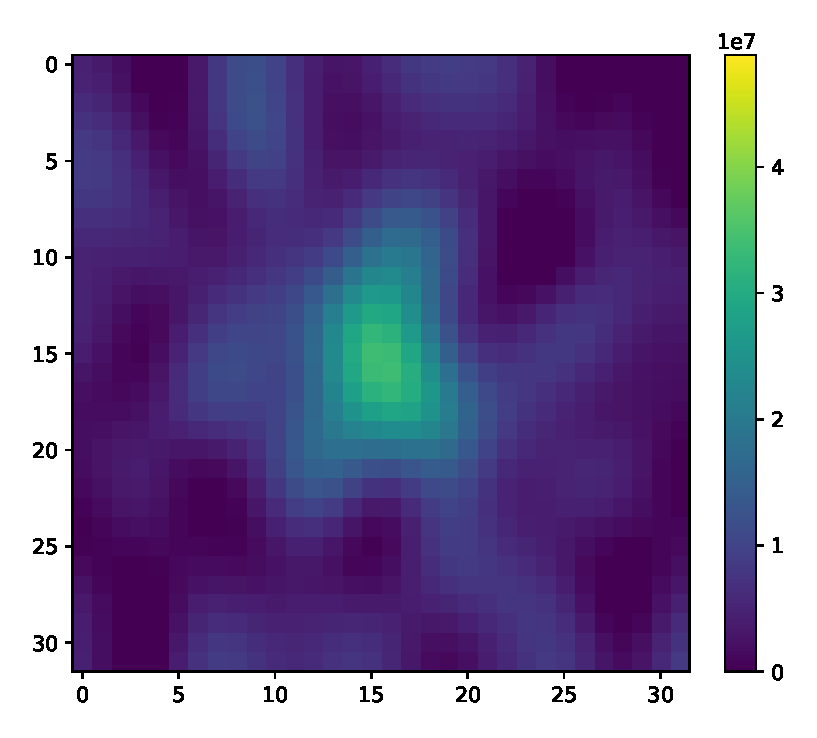
\includegraphics[width=\textwidth]{figures/06_results/gaussian_plume_example/munich/bp_dct_snr_20_db.eps}
        \caption{DCT}
    \end{subfigure}    
    \begin{subfigure}[b]{0.32\textwidth}
        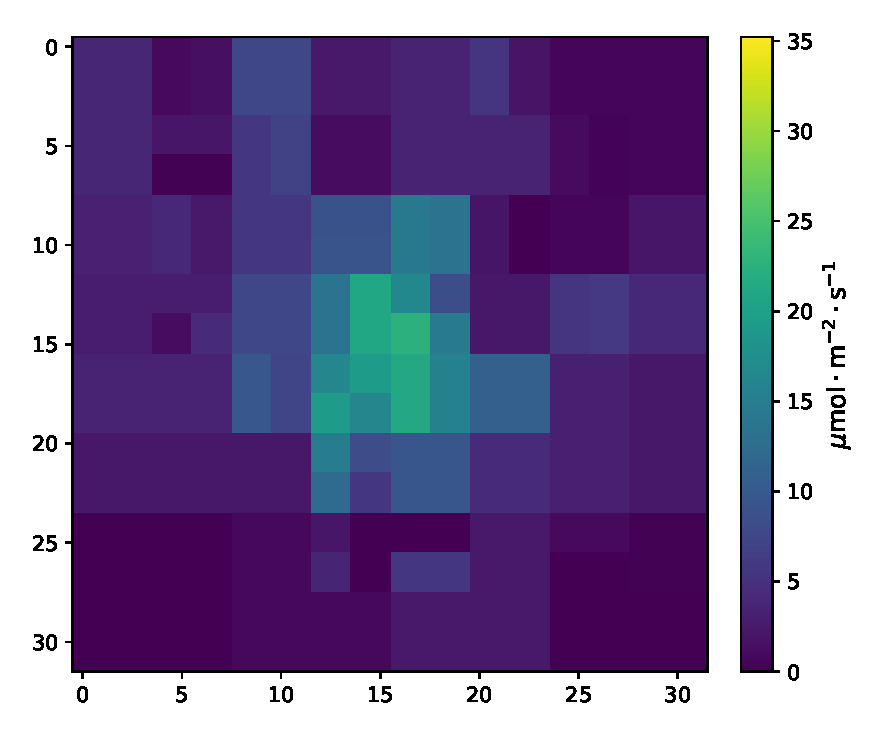
\includegraphics[width=\textwidth]{figures/06_results/gaussian_plume_example/munich/bp_dwt_snr_20_db.eps}
        \caption{DWT}
    \end{subfigure}
    \begin{subfigure}[b]{0.32\textwidth}
        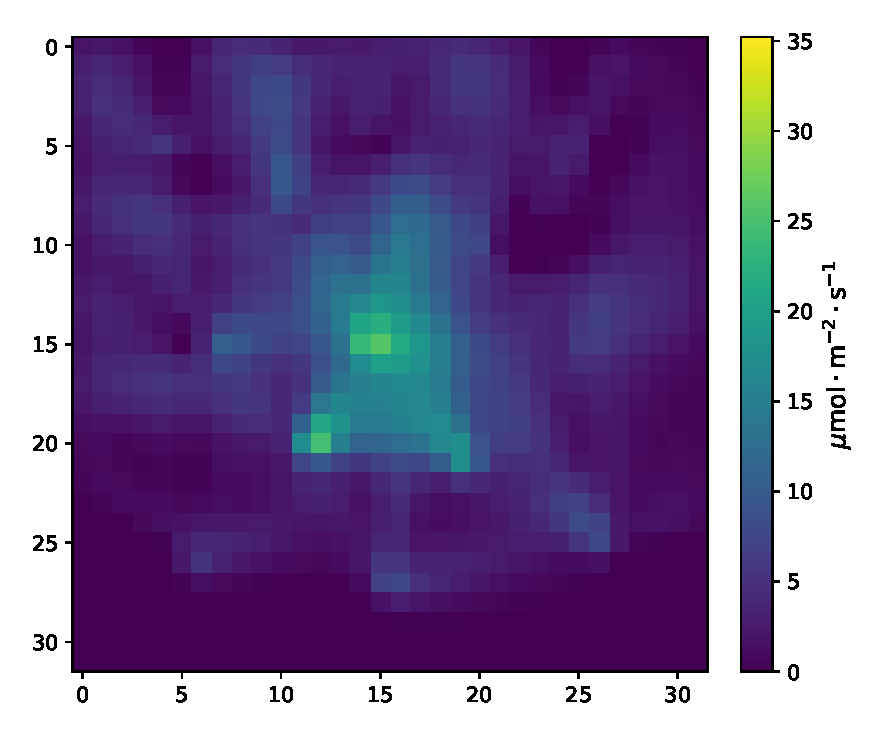
\includegraphics[width=\textwidth]{figures/06_results/gaussian_plume_example/munich/least_squares_snr_20_db.eps}
        \caption{LS}
    \end{subfigure}
    \caption{Target Munich}
\end{figure}
The results are reported in the following table.
This also includes the other models that performed worse than the 2048 one.

\section{Composition Into Sectors}

